%% Kortsett fra mattelab.no – laget automatisk av bygg.py. Rediger gjerne til eget bruk.
%% Kompiler med lualatex.
\documentclass[11pt,a4paper]{article}
\usepackage[norsk]{babel}
\usepackage[a4paper,margin=1.2cm,bottom=1.7cm]{geometry}
\usepackage{fontspec}
\usepackage{unicode-math}
\setmainfont{TeX Gyre Pagella}
\setsansfont{TeX Gyre Heros}[Scale=MatchLowercase]
\setmathfont{TeX Gyre Pagella Math}
\usepackage{xcolor}
\definecolor{blekk}{HTML}{16213A}
\definecolor{dempet}{HTML}{566077}
\definecolor{m1}{HTML}{2F4AB0}
\usepackage{tikz}
\usepackage{qrcode}
\usepackage{fancyhdr}
\usepackage[hidelinks]{hyperref}
\pdfvariable suppressoptionalinfo \numexpr 1+2+4+8+16+32+64+128+256+512\relax
\setlength{\parindent}{0pt}
\setlength{\parskip}{0pt}
\pagestyle{fancy}
\fancyhf{}
\renewcommand{\headrulewidth}{0pt}
\fancyfoot[L]{\sffamily\footnotesize\color{dempet}mattelab.no · Brøk, figur, desimaltall og prosent · kortsett K1}
\fancyfoot[R]{\sffamily\footnotesize\color{dempet}Side \thepage}
\begin{document}
\begin{minipage}[t]{0.8\linewidth}\vspace{0pt}
{\sffamily\small\color{dempet}Kortsett K1 · 1T · mattelab.no}\par\vspace{0.25em}
{\fontsize{20}{24}\selectfont\bfseries Brøk, figur, desimaltall og prosent}\par\vspace{0.5em}
Finn fire og fire kort som viser samme tall: en brøk, en figur, et desimaltall og en prosent.\par\vspace{0.4em}{\small\color{dempet}Klipp langs de stiplede linjene. Koden nede i hjørnet (K1-01, K1-02, …) viser hvilket sett kortet hører til.}
\end{minipage}\hfill
\begin{minipage}[t]{0.15\linewidth}\vspace{0pt}\raggedleft
\qrcode[height=1.9cm]{https://mattelab.no/varierende/brok-desimal-prosent.html}
\end{minipage}\par\vspace{0.8em}

\noindent\begin{tikzpicture}
\useasboundingbox (0,0) rectangle (6.19,4.0);
\node[text width=5.29cm, align=center, font=\Large] at (3.095,2.08) {$1{,}25$};
\draw[black!45, line width=0.4pt, dash pattern=on 3pt off 2.5pt] (0,0) rectangle (6.19,4.0);
\node[anchor=south east, font=\sffamily\scriptsize, text=black!55, inner sep=0pt] at (6.04,0.14) {K1-01};
\end{tikzpicture}%
\begin{tikzpicture}
\useasboundingbox (0,0) rectangle (6.19,4.0);
\node[text width=5.29cm, align=center, font=\Large] at (3.095,2.08) {$0{,}35$};
\draw[black!45, line width=0.4pt, dash pattern=on 3pt off 2.5pt] (0,0) rectangle (6.19,4.0);
\node[anchor=south east, font=\sffamily\scriptsize, text=black!55, inner sep=0pt] at (6.04,0.14) {K1-02};
\end{tikzpicture}%
\begin{tikzpicture}
\useasboundingbox (0,0) rectangle (6.19,4.0);
\node[text width=5.29cm, align=center, font=\Large] at (3.095,2.08) {$125\,\%$};
\draw[black!45, line width=0.4pt, dash pattern=on 3pt off 2.5pt] (0,0) rectangle (6.19,4.0);
\node[anchor=south east, font=\sffamily\scriptsize, text=black!55, inner sep=0pt] at (6.04,0.14) {K1-03};
\end{tikzpicture}%
\par\nointerlineskip
\noindent\begin{tikzpicture}
\useasboundingbox (0,0) rectangle (6.19,4.0);
\node[text width=5.29cm, align=center, font=\Large] at (3.095,2.08) {$75\,\%$};
\draw[black!45, line width=0.4pt, dash pattern=on 3pt off 2.5pt] (0,0) rectangle (6.19,4.0);
\node[anchor=south east, font=\sffamily\scriptsize, text=black!55, inner sep=0pt] at (6.04,0.14) {K1-04};
\end{tikzpicture}%
\begin{tikzpicture}
\useasboundingbox (0,0) rectangle (6.19,4.0);
\node[text width=5.29cm, align=center, font=\Large] at (3.095,2.08) {$\dfrac{1}{8}$};
\draw[black!45, line width=0.4pt, dash pattern=on 3pt off 2.5pt] (0,0) rectangle (6.19,4.0);
\node[anchor=south east, font=\sffamily\scriptsize, text=black!55, inner sep=0pt] at (6.04,0.14) {K1-05};
\end{tikzpicture}%
\begin{tikzpicture}
\useasboundingbox (0,0) rectangle (6.19,4.0);
\node[text width=5.29cm, align=center, font=\Large] at (3.095,2.08) {$\dfrac{1}{4}$};
\draw[black!45, line width=0.4pt, dash pattern=on 3pt off 2.5pt] (0,0) rectangle (6.19,4.0);
\node[anchor=south east, font=\sffamily\scriptsize, text=black!55, inner sep=0pt] at (6.04,0.14) {K1-06};
\end{tikzpicture}%
\par\nointerlineskip
\noindent\begin{tikzpicture}
\useasboundingbox (0,0) rectangle (6.19,4.0);
\node[text width=5.29cm, align=center, font=\Large] at (3.095,2.08) {$35\,\%$};
\draw[black!45, line width=0.4pt, dash pattern=on 3pt off 2.5pt] (0,0) rectangle (6.19,4.0);
\node[anchor=south east, font=\sffamily\scriptsize, text=black!55, inner sep=0pt] at (6.04,0.14) {K1-07};
\end{tikzpicture}%
\begin{tikzpicture}
\useasboundingbox (0,0) rectangle (6.19,4.0);
\node[text width=5.29cm, align=center, font=\Large] at (3.095,2.08) {$\dfrac{3}{10}$};
\draw[black!45, line width=0.4pt, dash pattern=on 3pt off 2.5pt] (0,0) rectangle (6.19,4.0);
\node[anchor=south east, font=\sffamily\scriptsize, text=black!55, inner sep=0pt] at (6.04,0.14) {K1-08};
\end{tikzpicture}%
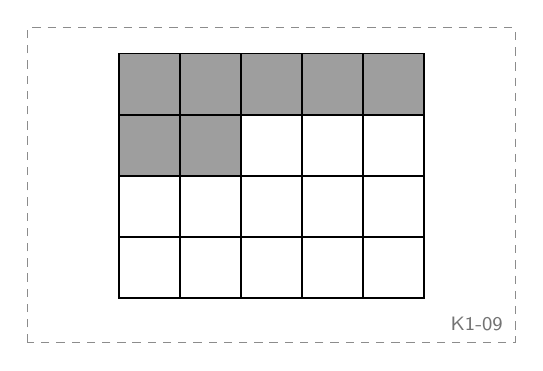
\begin{tikzpicture}
\useasboundingbox (0,0) rectangle (6.19,4.0);
\path[fill=black!38, draw=black, line width=0.6pt] (1.158,2.895) rectangle (1.933,3.67);
\path[fill=black!38, draw=black, line width=0.6pt] (1.933,2.895) rectangle (2.708,3.67);
\path[fill=black!38, draw=black, line width=0.6pt] (2.708,2.895) rectangle (3.483,3.67);
\path[fill=black!38, draw=black, line width=0.6pt] (3.483,2.895) rectangle (4.258,3.67);
\path[fill=black!38, draw=black, line width=0.6pt] (4.258,2.895) rectangle (5.033,3.67);
\path[fill=black!38, draw=black, line width=0.6pt] (1.158,2.12) rectangle (1.933,2.895);
\path[fill=black!38, draw=black, line width=0.6pt] (1.933,2.12) rectangle (2.708,2.895);
\path[fill=white, draw=black, line width=0.6pt] (2.708,2.12) rectangle (3.483,2.895);
\path[fill=white, draw=black, line width=0.6pt] (3.483,2.12) rectangle (4.258,2.895);
\path[fill=white, draw=black, line width=0.6pt] (4.258,2.12) rectangle (5.033,2.895);
\path[fill=white, draw=black, line width=0.6pt] (1.158,1.345) rectangle (1.933,2.12);
\path[fill=white, draw=black, line width=0.6pt] (1.933,1.345) rectangle (2.708,2.12);
\path[fill=white, draw=black, line width=0.6pt] (2.708,1.345) rectangle (3.483,2.12);
\path[fill=white, draw=black, line width=0.6pt] (3.483,1.345) rectangle (4.258,2.12);
\path[fill=white, draw=black, line width=0.6pt] (4.258,1.345) rectangle (5.033,2.12);
\path[fill=white, draw=black, line width=0.6pt] (1.158,0.57) rectangle (1.933,1.345);
\path[fill=white, draw=black, line width=0.6pt] (1.933,0.57) rectangle (2.708,1.345);
\path[fill=white, draw=black, line width=0.6pt] (2.708,0.57) rectangle (3.483,1.345);
\path[fill=white, draw=black, line width=0.6pt] (3.483,0.57) rectangle (4.258,1.345);
\path[fill=white, draw=black, line width=0.6pt] (4.258,0.57) rectangle (5.033,1.345);
\draw[black!45, line width=0.4pt, dash pattern=on 3pt off 2.5pt] (0,0) rectangle (6.19,4.0);
\node[anchor=south east, font=\sffamily\scriptsize, text=black!55, inner sep=0pt] at (6.04,0.14) {K1-09};
\end{tikzpicture}%
\par\nointerlineskip
\noindent\begin{tikzpicture}
\useasboundingbox (0,0) rectangle (6.19,4.0);
\node[text width=5.29cm, align=center, font=\Large] at (3.095,2.08) {$0{,}\overline{6}$};
\draw[black!45, line width=0.4pt, dash pattern=on 3pt off 2.5pt] (0,0) rectangle (6.19,4.0);
\node[anchor=south east, font=\sffamily\scriptsize, text=black!55, inner sep=0pt] at (6.04,0.14) {K1-10};
\end{tikzpicture}%
\begin{tikzpicture}
\useasboundingbox (0,0) rectangle (6.19,4.0);
\node[text width=5.29cm, align=center, font=\Large] at (3.095,2.08) {$\dfrac{2}{5}$};
\draw[black!45, line width=0.4pt, dash pattern=on 3pt off 2.5pt] (0,0) rectangle (6.19,4.0);
\node[anchor=south east, font=\sffamily\scriptsize, text=black!55, inner sep=0pt] at (6.04,0.14) {K1-11};
\end{tikzpicture}%
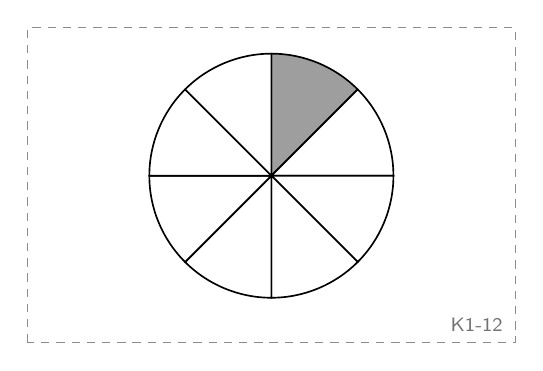
\begin{tikzpicture}
\useasboundingbox (0,0) rectangle (6.19,4.0);
\path[fill=black!38, draw=black, line width=0.6pt] (3.095,2.12) -- ++(45:1.55) arc[start angle=45, end angle=90, radius=1.55] -- cycle;
\path[fill=white, draw=black, line width=0.6pt] (3.095,2.12) -- ++(0:1.55) arc[start angle=0, end angle=45, radius=1.55] -- cycle;
\path[fill=white, draw=black, line width=0.6pt] (3.095,2.12) -- ++(-45:1.55) arc[start angle=-45, end angle=0, radius=1.55] -- cycle;
\path[fill=white, draw=black, line width=0.6pt] (3.095,2.12) -- ++(-90:1.55) arc[start angle=-90, end angle=-45, radius=1.55] -- cycle;
\path[fill=white, draw=black, line width=0.6pt] (3.095,2.12) -- ++(-135:1.55) arc[start angle=-135, end angle=-90, radius=1.55] -- cycle;
\path[fill=white, draw=black, line width=0.6pt] (3.095,2.12) -- ++(-180:1.55) arc[start angle=-180, end angle=-135, radius=1.55] -- cycle;
\path[fill=white, draw=black, line width=0.6pt] (3.095,2.12) -- ++(-225:1.55) arc[start angle=-225, end angle=-180, radius=1.55] -- cycle;
\path[fill=white, draw=black, line width=0.6pt] (3.095,2.12) -- ++(-270:1.55) arc[start angle=-270, end angle=-225, radius=1.55] -- cycle;
\draw[black!45, line width=0.4pt, dash pattern=on 3pt off 2.5pt] (0,0) rectangle (6.19,4.0);
\node[anchor=south east, font=\sffamily\scriptsize, text=black!55, inner sep=0pt] at (6.04,0.14) {K1-12};
\end{tikzpicture}%
\par\nointerlineskip
\noindent\begin{tikzpicture}
\useasboundingbox (0,0) rectangle (6.19,4.0);
\node[text width=5.29cm, align=center, font=\Large] at (3.095,2.08) {$30\,\%$};
\draw[black!45, line width=0.4pt, dash pattern=on 3pt off 2.5pt] (0,0) rectangle (6.19,4.0);
\node[anchor=south east, font=\sffamily\scriptsize, text=black!55, inner sep=0pt] at (6.04,0.14) {K1-13};
\end{tikzpicture}%
\begin{tikzpicture}
\useasboundingbox (0,0) rectangle (6.19,4.0);
\node[text width=5.29cm, align=center, font=\Large] at (3.095,2.08) {$0{,}25$};
\draw[black!45, line width=0.4pt, dash pattern=on 3pt off 2.5pt] (0,0) rectangle (6.19,4.0);
\node[anchor=south east, font=\sffamily\scriptsize, text=black!55, inner sep=0pt] at (6.04,0.14) {K1-14};
\end{tikzpicture}%
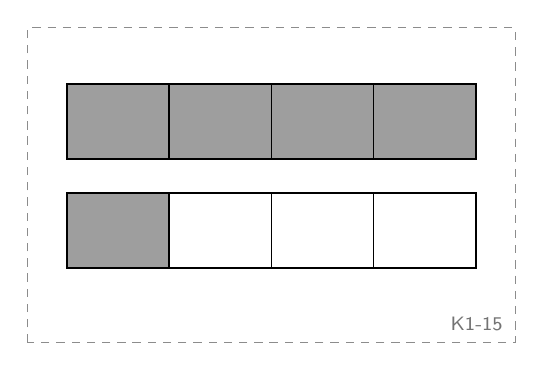
\begin{tikzpicture}
\useasboundingbox (0,0) rectangle (6.19,4.0);
\path[fill=black!38, draw=black, line width=0.6pt] (0.5,2.336) rectangle (1.798,3.288);
\path[fill=black!38, draw=black, line width=0.6pt] (1.798,2.336) rectangle (3.095,3.288);
\path[fill=black!38, draw=black, line width=0.6pt] (3.095,2.336) rectangle (4.393,3.288);
\path[fill=black!38, draw=black, line width=0.6pt] (4.393,2.336) rectangle (5.69,3.288);
\path[fill=black!38, draw=black, line width=0.6pt] (0.5,0.952) rectangle (1.798,1.904);
\path[fill=white, draw=black, line width=0.6pt] (1.798,0.952) rectangle (3.095,1.904);
\path[fill=white, draw=black, line width=0.6pt] (3.095,0.952) rectangle (4.393,1.904);
\path[fill=white, draw=black, line width=0.6pt] (4.393,0.952) rectangle (5.69,1.904);
\draw[black!45, line width=0.4pt, dash pattern=on 3pt off 2.5pt] (0,0) rectangle (6.19,4.0);
\node[anchor=south east, font=\sffamily\scriptsize, text=black!55, inner sep=0pt] at (6.04,0.14) {K1-15};
\end{tikzpicture}%
\par\nointerlineskip
\noindent\begin{tikzpicture}
\useasboundingbox (0,0) rectangle (6.19,4.0);
\node[text width=5.29cm, align=center, font=\Large] at (3.095,2.08) {$25\,\%$};
\draw[black!45, line width=0.4pt, dash pattern=on 3pt off 2.5pt] (0,0) rectangle (6.19,4.0);
\node[anchor=south east, font=\sffamily\scriptsize, text=black!55, inner sep=0pt] at (6.04,0.14) {K1-16};
\end{tikzpicture}%
\begin{tikzpicture}
\useasboundingbox (0,0) rectangle (6.19,4.0);
\node[text width=5.29cm, align=center, font=\Large] at (3.095,2.08) {$\dfrac{2}{3}$};
\draw[black!45, line width=0.4pt, dash pattern=on 3pt off 2.5pt] (0,0) rectangle (6.19,4.0);
\node[anchor=south east, font=\sffamily\scriptsize, text=black!55, inner sep=0pt] at (6.04,0.14) {K1-17};
\end{tikzpicture}%
\begin{tikzpicture}
\useasboundingbox (0,0) rectangle (6.19,4.0);
\node[text width=5.29cm, align=center, font=\Large] at (3.095,2.08) {$\dfrac{3}{4}$};
\draw[black!45, line width=0.4pt, dash pattern=on 3pt off 2.5pt] (0,0) rectangle (6.19,4.0);
\node[anchor=south east, font=\sffamily\scriptsize, text=black!55, inner sep=0pt] at (6.04,0.14) {K1-18};
\end{tikzpicture}%
\par\nointerlineskip
\noindent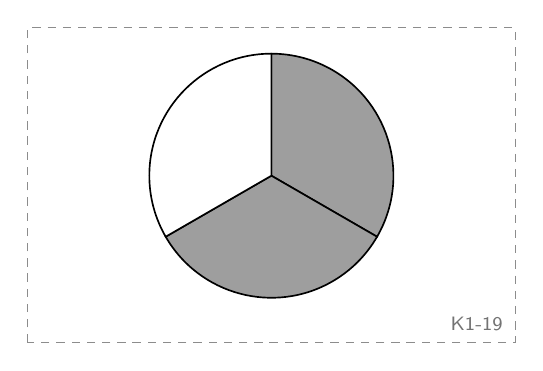
\begin{tikzpicture}
\useasboundingbox (0,0) rectangle (6.19,4.0);
\path[fill=black!38, draw=black, line width=0.6pt] (3.095,2.12) -- ++(-30:1.55) arc[start angle=-30, end angle=90, radius=1.55] -- cycle;
\path[fill=black!38, draw=black, line width=0.6pt] (3.095,2.12) -- ++(-150:1.55) arc[start angle=-150, end angle=-30, radius=1.55] -- cycle;
\path[fill=white, draw=black, line width=0.6pt] (3.095,2.12) -- ++(-270:1.55) arc[start angle=-270, end angle=-150, radius=1.55] -- cycle;
\draw[black!45, line width=0.4pt, dash pattern=on 3pt off 2.5pt] (0,0) rectangle (6.19,4.0);
\node[anchor=south east, font=\sffamily\scriptsize, text=black!55, inner sep=0pt] at (6.04,0.14) {K1-19};
\end{tikzpicture}%
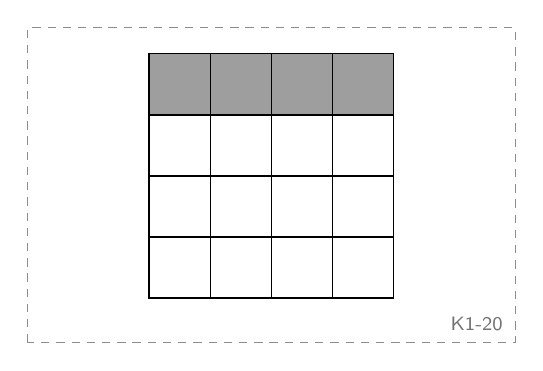
\begin{tikzpicture}
\useasboundingbox (0,0) rectangle (6.19,4.0);
\path[fill=black!38, draw=black, line width=0.6pt] (1.545,2.895) rectangle (2.32,3.67);
\path[fill=black!38, draw=black, line width=0.6pt] (2.32,2.895) rectangle (3.095,3.67);
\path[fill=black!38, draw=black, line width=0.6pt] (3.095,2.895) rectangle (3.87,3.67);
\path[fill=black!38, draw=black, line width=0.6pt] (3.87,2.895) rectangle (4.645,3.67);
\path[fill=white, draw=black, line width=0.6pt] (1.545,2.12) rectangle (2.32,2.895);
\path[fill=white, draw=black, line width=0.6pt] (2.32,2.12) rectangle (3.095,2.895);
\path[fill=white, draw=black, line width=0.6pt] (3.095,2.12) rectangle (3.87,2.895);
\path[fill=white, draw=black, line width=0.6pt] (3.87,2.12) rectangle (4.645,2.895);
\path[fill=white, draw=black, line width=0.6pt] (1.545,1.345) rectangle (2.32,2.12);
\path[fill=white, draw=black, line width=0.6pt] (2.32,1.345) rectangle (3.095,2.12);
\path[fill=white, draw=black, line width=0.6pt] (3.095,1.345) rectangle (3.87,2.12);
\path[fill=white, draw=black, line width=0.6pt] (3.87,1.345) rectangle (4.645,2.12);
\path[fill=white, draw=black, line width=0.6pt] (1.545,0.57) rectangle (2.32,1.345);
\path[fill=white, draw=black, line width=0.6pt] (2.32,0.57) rectangle (3.095,1.345);
\path[fill=white, draw=black, line width=0.6pt] (3.095,0.57) rectangle (3.87,1.345);
\path[fill=white, draw=black, line width=0.6pt] (3.87,0.57) rectangle (4.645,1.345);
\draw[black!45, line width=0.4pt, dash pattern=on 3pt off 2.5pt] (0,0) rectangle (6.19,4.0);
\node[anchor=south east, font=\sffamily\scriptsize, text=black!55, inner sep=0pt] at (6.04,0.14) {K1-20};
\end{tikzpicture}%
\begin{tikzpicture}
\useasboundingbox (0,0) rectangle (6.19,4.0);
\node[text width=5.29cm, align=center, font=\Large] at (3.095,2.08) {$66\tfrac{2}{3}\,\%$};
\draw[black!45, line width=0.4pt, dash pattern=on 3pt off 2.5pt] (0,0) rectangle (6.19,4.0);
\node[anchor=south east, font=\sffamily\scriptsize, text=black!55, inner sep=0pt] at (6.04,0.14) {K1-21};
\end{tikzpicture}%
\par\nointerlineskip
\noindent\begin{tikzpicture}
\useasboundingbox (0,0) rectangle (6.19,4.0);
\node[text width=5.29cm, align=center, font=\Large] at (3.095,2.08) {$0{,}125$};
\draw[black!45, line width=0.4pt, dash pattern=on 3pt off 2.5pt] (0,0) rectangle (6.19,4.0);
\node[anchor=south east, font=\sffamily\scriptsize, text=black!55, inner sep=0pt] at (6.04,0.14) {K1-22};
\end{tikzpicture}%
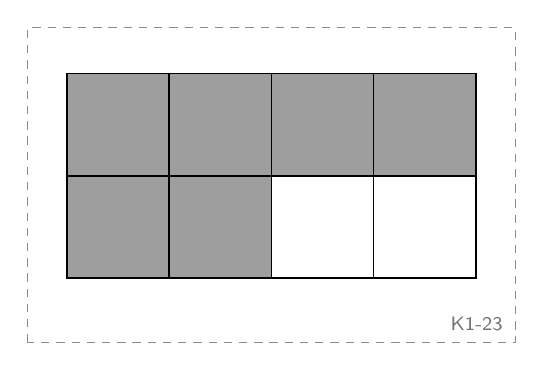
\begin{tikzpicture}
\useasboundingbox (0,0) rectangle (6.19,4.0);
\path[fill=black!38, draw=black, line width=0.6pt] (0.5,2.12) rectangle (1.798,3.418);
\path[fill=black!38, draw=black, line width=0.6pt] (1.798,2.12) rectangle (3.095,3.418);
\path[fill=black!38, draw=black, line width=0.6pt] (3.095,2.12) rectangle (4.393,3.418);
\path[fill=black!38, draw=black, line width=0.6pt] (4.393,2.12) rectangle (5.69,3.418);
\path[fill=black!38, draw=black, line width=0.6pt] (0.5,0.823) rectangle (1.798,2.12);
\path[fill=black!38, draw=black, line width=0.6pt] (1.798,0.823) rectangle (3.095,2.12);
\path[fill=white, draw=black, line width=0.6pt] (3.095,0.823) rectangle (4.393,2.12);
\path[fill=white, draw=black, line width=0.6pt] (4.393,0.823) rectangle (5.69,2.12);
\draw[black!45, line width=0.4pt, dash pattern=on 3pt off 2.5pt] (0,0) rectangle (6.19,4.0);
\node[anchor=south east, font=\sffamily\scriptsize, text=black!55, inner sep=0pt] at (6.04,0.14) {K1-23};
\end{tikzpicture}%
\begin{tikzpicture}
\useasboundingbox (0,0) rectangle (6.19,4.0);
\node[text width=5.29cm, align=center, font=\Large] at (3.095,2.08) {$12{,}5\,\%$};
\draw[black!45, line width=0.4pt, dash pattern=on 3pt off 2.5pt] (0,0) rectangle (6.19,4.0);
\node[anchor=south east, font=\sffamily\scriptsize, text=black!55, inner sep=0pt] at (6.04,0.14) {K1-24};
\end{tikzpicture}%
\par\nointerlineskip
\noindent\begin{tikzpicture}
\useasboundingbox (0,0) rectangle (6.19,4.0);
\node[text width=5.29cm, align=center, font=\Large] at (3.095,2.08) {$0{,}3$};
\draw[black!45, line width=0.4pt, dash pattern=on 3pt off 2.5pt] (0,0) rectangle (6.19,4.0);
\node[anchor=south east, font=\sffamily\scriptsize, text=black!55, inner sep=0pt] at (6.04,0.14) {K1-25};
\end{tikzpicture}%
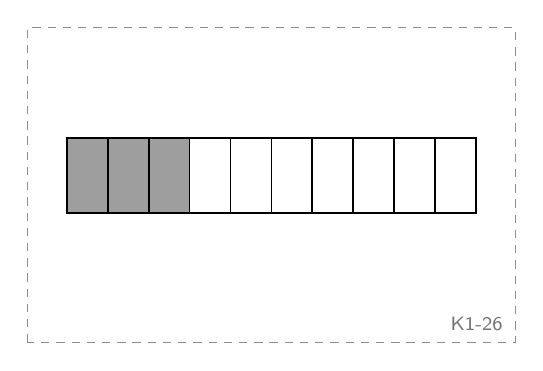
\begin{tikzpicture}
\useasboundingbox (0,0) rectangle (6.19,4.0);
\path[fill=black!38, draw=black, line width=0.6pt] (0.5,1.644) rectangle (1.019,2.596);
\path[fill=black!38, draw=black, line width=0.6pt] (1.019,1.644) rectangle (1.538,2.596);
\path[fill=black!38, draw=black, line width=0.6pt] (1.538,1.644) rectangle (2.057,2.596);
\path[fill=white, draw=black, line width=0.6pt] (2.057,1.644) rectangle (2.576,2.596);
\path[fill=white, draw=black, line width=0.6pt] (2.576,1.644) rectangle (3.095,2.596);
\path[fill=white, draw=black, line width=0.6pt] (3.095,1.644) rectangle (3.614,2.596);
\path[fill=white, draw=black, line width=0.6pt] (3.614,1.644) rectangle (4.133,2.596);
\path[fill=white, draw=black, line width=0.6pt] (4.133,1.644) rectangle (4.652,2.596);
\path[fill=white, draw=black, line width=0.6pt] (4.652,1.644) rectangle (5.171,2.596);
\path[fill=white, draw=black, line width=0.6pt] (5.171,1.644) rectangle (5.69,2.596);
\draw[black!45, line width=0.4pt, dash pattern=on 3pt off 2.5pt] (0,0) rectangle (6.19,4.0);
\node[anchor=south east, font=\sffamily\scriptsize, text=black!55, inner sep=0pt] at (6.04,0.14) {K1-26};
\end{tikzpicture}%
\begin{tikzpicture}
\useasboundingbox (0,0) rectangle (6.19,4.0);
\node[text width=5.29cm, align=center, font=\Large] at (3.095,2.08) {$0{,}4$};
\draw[black!45, line width=0.4pt, dash pattern=on 3pt off 2.5pt] (0,0) rectangle (6.19,4.0);
\node[anchor=south east, font=\sffamily\scriptsize, text=black!55, inner sep=0pt] at (6.04,0.14) {K1-27};
\end{tikzpicture}%
\par\nointerlineskip
\noindent\begin{tikzpicture}
\useasboundingbox (0,0) rectangle (6.19,4.0);
\node[text width=5.29cm, align=center, font=\Large] at (3.095,2.08) {$\dfrac{5}{4}$};
\draw[black!45, line width=0.4pt, dash pattern=on 3pt off 2.5pt] (0,0) rectangle (6.19,4.0);
\node[anchor=south east, font=\sffamily\scriptsize, text=black!55, inner sep=0pt] at (6.04,0.14) {K1-28};
\end{tikzpicture}%
\begin{tikzpicture}
\useasboundingbox (0,0) rectangle (6.19,4.0);
\node[text width=5.29cm, align=center, font=\Large] at (3.095,2.08) {$0{,}75$};
\draw[black!45, line width=0.4pt, dash pattern=on 3pt off 2.5pt] (0,0) rectangle (6.19,4.0);
\node[anchor=south east, font=\sffamily\scriptsize, text=black!55, inner sep=0pt] at (6.04,0.14) {K1-29};
\end{tikzpicture}%
\begin{tikzpicture}
\useasboundingbox (0,0) rectangle (6.19,4.0);
\node[text width=5.29cm, align=center, font=\Large] at (3.095,2.08) {$40\,\%$};
\draw[black!45, line width=0.4pt, dash pattern=on 3pt off 2.5pt] (0,0) rectangle (6.19,4.0);
\node[anchor=south east, font=\sffamily\scriptsize, text=black!55, inner sep=0pt] at (6.04,0.14) {K1-30};
\end{tikzpicture}%
\par\nointerlineskip
\noindent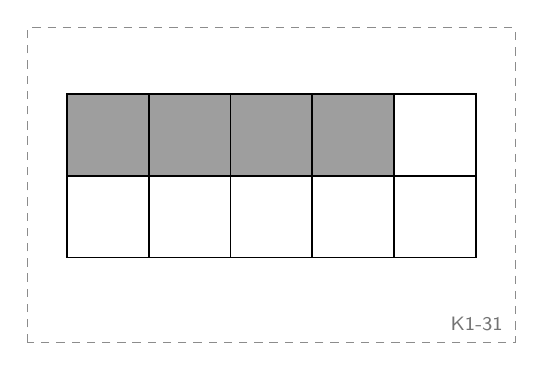
\begin{tikzpicture}
\useasboundingbox (0,0) rectangle (6.19,4.0);
\path[fill=black!38, draw=black, line width=0.6pt] (0.5,2.12) rectangle (1.538,3.158);
\path[fill=black!38, draw=black, line width=0.6pt] (1.538,2.12) rectangle (2.576,3.158);
\path[fill=black!38, draw=black, line width=0.6pt] (2.576,2.12) rectangle (3.614,3.158);
\path[fill=black!38, draw=black, line width=0.6pt] (3.614,2.12) rectangle (4.652,3.158);
\path[fill=white, draw=black, line width=0.6pt] (4.652,2.12) rectangle (5.69,3.158);
\path[fill=white, draw=black, line width=0.6pt] (0.5,1.082) rectangle (1.538,2.12);
\path[fill=white, draw=black, line width=0.6pt] (1.538,1.082) rectangle (2.576,2.12);
\path[fill=white, draw=black, line width=0.6pt] (2.576,1.082) rectangle (3.614,2.12);
\path[fill=white, draw=black, line width=0.6pt] (3.614,1.082) rectangle (4.652,2.12);
\path[fill=white, draw=black, line width=0.6pt] (4.652,1.082) rectangle (5.69,2.12);
\draw[black!45, line width=0.4pt, dash pattern=on 3pt off 2.5pt] (0,0) rectangle (6.19,4.0);
\node[anchor=south east, font=\sffamily\scriptsize, text=black!55, inner sep=0pt] at (6.04,0.14) {K1-31};
\end{tikzpicture}%
\begin{tikzpicture}
\useasboundingbox (0,0) rectangle (6.19,4.0);
\node[text width=5.29cm, align=center, font=\Large] at (3.095,2.08) {$\dfrac{7}{20}$};
\draw[black!45, line width=0.4pt, dash pattern=on 3pt off 2.5pt] (0,0) rectangle (6.19,4.0);
\node[anchor=south east, font=\sffamily\scriptsize, text=black!55, inner sep=0pt] at (6.04,0.14) {K1-32};
\end{tikzpicture}%
\begin{tikzpicture}
\useasboundingbox (0,0) rectangle (6.19,4.0);
\node[anchor=south east, font=\sffamily\scriptsize, text=black!40, inner sep=0pt] at (6.04,0.14) {Eget kort};
\draw[black!45, line width=0.4pt, dash pattern=on 3pt off 2.5pt] (0,0) rectangle (6.19,4.0);
\end{tikzpicture}%
\par\nointerlineskip
\noindent\begin{tikzpicture}
\useasboundingbox (0,0) rectangle (6.19,4.0);
\node[anchor=south east, font=\sffamily\scriptsize, text=black!40, inner sep=0pt] at (6.04,0.14) {Eget kort};
\draw[black!45, line width=0.4pt, dash pattern=on 3pt off 2.5pt] (0,0) rectangle (6.19,4.0);
\end{tikzpicture}%
\begin{tikzpicture}
\useasboundingbox (0,0) rectangle (6.19,4.0);
\node[anchor=south east, font=\sffamily\scriptsize, text=black!40, inner sep=0pt] at (6.04,0.14) {Eget kort};
\draw[black!45, line width=0.4pt, dash pattern=on 3pt off 2.5pt] (0,0) rectangle (6.19,4.0);
\end{tikzpicture}%
\begin{tikzpicture}
\useasboundingbox (0,0) rectangle (6.19,4.0);
\node[anchor=south east, font=\sffamily\scriptsize, text=black!40, inner sep=0pt] at (6.04,0.14) {Eget kort};
\draw[black!45, line width=0.4pt, dash pattern=on 3pt off 2.5pt] (0,0) rectangle (6.19,4.0);
\end{tikzpicture}%
\par\nointerlineskip
\end{document}
